\documentclass[11pt,a4paper]{article}

\usepackage{amsmath,amssymb,amsthm}
\usepackage{mathtools}
\usepackage{geometry}
\usepackage{xcolor}
\usepackage{hyperref}
\usepackage{graphicx}
\usepackage{booktabs}
\usepackage{microtype}
\usepackage{cleveref}

\geometry{margin=2.5cm}

\hypersetup{
  colorlinks=true,
  linkcolor=blue!60!black,
  citecolor=green!50!black,
  urlcolor=blue!70!black
}

\newtheorem{theorem}{Theorem}[section]
\newtheorem{proposition}[theorem]{Proposition}
\newtheorem{lemma}[theorem]{Lemma}
\newtheorem{corollary}[theorem]{Corollary}
\newtheorem{conjecture}[theorem]{Conjecture}
\theoremstyle{definition}
\newtheorem{definition}[theorem]{Definition}
\theoremstyle{remark}
\newtheorem{remark}[theorem]{Remark}

% Notation
\newcommand{\PSL}{\mathrm{PSL}(2,\mathbb{F}_q)}
\newcommand{\Sp}{\mathcal{S}_p}
\newcommand{\Ad}{\mathrm{Ad}}
\newcommand{\Pik}{\Pi_k}
\newcommand{\beff}{\beta_{\mathrm{eff}}}
\newcommand{\heff}{\hbar_{\mathrm{eff}}}
\newcommand{\Heff}{\hat{H}_{\mathrm{eff}}}
\newcommand{\spann}{\mathrm{span}}
\newcommand{\nov}{\mathrm{nov}}
\newcommand{\Pk}{\mathcal{P}_k}

\title{%
  \textbf{Projective Capacity and the Continuum Limit of Admissible Redundancy}\\[0.4em]
  \large From Discrete Path Fingerprints to Nonlinear Projected Dynamics
}

\author{%
  J\'{e}r\^{o}me Beau\\[0.3em]
  \small Independent Researcher; \texttt{jerome.beau@cosmochrony.org}
}

\date{March 2026}

\begin{document}

  \maketitle

  \begin{abstract}
    The Cosmochrony spectral cascade programme has progressively constrained the exponent~$\beta$
    governing the growth $p(n) \sim n^\beta$ of the effective relational valence.
    O4 established $\beta \leq 1$ from Born--Infeld saturation and the Cheeger isoperimetric
    inequality.
    O5 and O6 proved that vertex-level and fixed-representation fingerprints saturate within
    bounded BFS depth, independent of~$q$, and O6, Proposition~6.2 formalised this as a universal
    no-go: no fingerprint based on a fixed finite-dimensional representation can produce the
    power-law decay $R_n \sim p(n)^{-\alpha}$ required to close on $\beta^* \in (0.09, 0.13)$.

    The present paper introduces the bridge between this discrete obstruction and the nonlinear
    projected dynamics derived in Appendix~B.14 of the Cosmochrony white paper~\cite{Cosmochrony},
    where the finite local spectral admissible capacity $\Sigma(x,t)$ and the projective
    occupancy $\eta = |\psi|^2/\Sigma$ give rise to the effective Gross--Pitaevskii equation
    with coupling $g = \gamma/\Sigma$ encoding projective saturation pressure.

    We construct the \emph{discrete projective capacity} $\Sigma_n(x)$ from path fingerprints
    of depth~$k$ via the effective novelty of each path relative to the already-spanned
    fingerprint subspace.
    We define the discrete projective occupancy $\eta_n(x) = |\psi_n(x)|^2/\Sigma_n(x)$ and
    establish, exactly in a reduced filling model, the \emph{state law}
    $R_n^{(k)}(x) \approx \Phi(\eta_n(x))$,
    where $\Phi(\eta) = 1/\sqrt{1+\eta^2}$ satisfies $\Phi(0)=1$, $\Phi(\eta)\to 0$ as
    $\eta \to \infty$, and $\Phi' < 0$.
    Numerical support is provided by reduced-model simulations for ambient dimensions
    $D \in \{9,27,81\}$ (corresponding to $k=2,3,4$ adjoint fingerprints), with the LPS graph
    $X_{5,13}$ included as a reference confirming the bounded-depth pre-saturation predicted by O6.
    We show that $\beta$ can be reread as the exponent governing the growth of~$\Sigma_n$ along the cascade.
    The Gross--Pitaevskii coupling of B.14 is then identified as the continuum image of the
    discrete saturation pressure $\gamma\eta_n\psi_n$.

    The central identification $R_n^{(k)} \approx \Phi(\eta_n)$ is established exactly in the
    reduced model and supported numerically; its full graph-theoretic derivation is left as an open problem.
    This reframes the sequence of no-go results of O5--O6 as a positive convergence statement:
    admissible redundancy is not merely a combinatorial obstruction count, but the microscopic
    precursor of a continuous projective dynamics whose nonlinear structure is already
    determined by the framework.
  \end{abstract}

  \paragraph{Keywords.}
    projective capacity, admissible redundancy, cascade exponent, nonlinear dynamics, continuum limit,
    spectral admissibility, bounded-depth saturation, coarse-graining, non-injective projection,
    Gross–Pitaevskii equation, effective coupling, emergent dynamics, capacity scaling

    \clearpage
    \tableofcontents

    \clearpage

  \section{Introduction}
  \label{sec:intro}

  \subsection{The hierarchy of obstructions O4--O6}
    \label{ssec:hierarchy}

    The O-series of papers in the Cosmochrony spectral cascade programme has pursued a single
    structural question: what mechanism is responsible for the smallness of the cascade exponent
    $\beta$, defined by the growth law $p(n) \sim n^\beta$ of the effective relational valence
    along the BFS cascade on LPS Ramanujan graphs $X_{p,q}$?
    The phenomenological window $\beta^* \in (0.09, 0.13)$ is fixed by the charged lepton
    mass ratios in O3~\cite{Beau2026a7}.
    Three successive structural results have been established.

    \paragraph{O4~\cite{Beau2026a8}.}
      The bounded-flux constraint $|\partial_t\chi_v| \leq c_{\mathrm{BI}}$, inherited from Born--Infeld
      saturation, combined with the Cheeger isoperimetric inequality for Ramanujan--LPS graphs,
      gives $\Delta p(n) \lesssim c_{\mathrm{BI}}\sqrt{p(n)}$, hence the structural upper bound $\beta \leq 1$
      (in the rescaled convention of~\cite{Beau2026a8}).
      This bound excludes super-quadratic growth but does not explain the gap to $\beta^* \approx 0.10$.

    \paragraph{O5~\cite{Beau2026a9}.}
      The vertex-based admissible span satisfies $\dim\Pi_A(S_n) \leq |\mathrm{Cl}(G)| = O(q)$,
      giving a saturation threshold $|S^*| = O(q)$ beyond which no vertex contributes a new
      admissible direction.
      No vertex-level mechanism can produce $R_n \sim p(n)^{-\alpha}$.

    \paragraph{O6~\cite{Beau2026a10}.}
      The Steinberg-matrix fingerprint of ambient dimension $O(q^2)$ saturates at BFS depth~6
      for all $q \in \{29,41,61\}$, independent of~$q$.
      Proposition~6.2 of~\cite{Beau2026a10} proves the universal no-go: for any fixed
      finite-dimensional representation $\rho$, there exists $k^*(\rho,p) < \infty$, independent
      of~$q$, such that $\dim\Pi_\rho(S_n)$ stabilises for $n \geq k^*$.
      The mechanism is the Hecke operator action of the LPS generators $\Omega_p$ on
      $\mathrm{End}(V_\rho)$, which spans the full endomorphism algebra within bounded depth.

      The logical consequence is unambiguous: overcoming the O6 obstruction requires a fingerprint
      space that grows with BFS depth, or a genuinely dynamical memory mechanism.
      O6, Corollary~4.4 sets the target precisely: construct a fingerprint with a power-law decay
      $R_n \sim p(n)^{-\alpha}$, $\alpha \in [7.4, 10.6]$.

      \begin{remark}[Scope of O7 relative to O6]
        \label{rem:o7-scope}
        O7 does not attempt to overcome the representation-theoretic obstruction identified in O6.
        It reformulates it in terms of a coarse-grained capacity $\Sigma_n(x)$ whose dynamics
        admits a continuous description.
        The obstruction is not circumvented but \emph{reinterpreted}: the bounded-depth saturation
        of O6 is the microscopic signature of a projective capacity exhaustion that, in the
        continuum limit, takes the form of the nonlinear dynamics of Appendix~B.14.
      \end{remark}

  \subsection{What Appendix~B.14 of the white paper brings}
  \label{ssec:b14}

  Independently of the discrete O-series, Appendix~B.14 of the Cosmochrony white
  paper~\cite{Cosmochrony} derives, in the continuous projected dynamics, the following
  result starting from Proposition~B.1 of~\cite{Cosmochrony}:
  \begin{equation}
    \label{eq:schrodinger-eff}
    i\heff\,\partial_t\psi = \Heff\psi + N_{\Pi,\mathrm{BI}}[\psi].
  \end{equation}
  In the regime of non-negligible projective occupancy $\eta = |\psi|^2/\Sigma \not\ll 1$,
  where $\Sigma(x,t) = \sum_n w_n A_n^{\max}$ is the local spectral admissible capacity,
  the leading correction is:
  \begin{equation}
    \label{eq:GP}
    i\heff\,\partial_t\psi
    = -\kappa\,\Delta_g\psi + V_{\mathrm{eff}}\psi
    + \frac{\gamma}{\Sigma(x,t)}\,|\psi|^2\psi + O(|\psi|^4\psi).
  \end{equation}
  The coupling $g(x,t) = \gamma/\Sigma(x,t)$ is not postulated but derived from the finite local
  admissible capacity.
  B.14 identifies three regimes: $\eta \ll 1$ (linear Schr\"{o}dinger), $\eta \lesssim 1$
  (Gross--Pitaevskii, possible soliton formation), $\eta \to 1$ (near-saturation boundary).

  These regimes at the continuous level have no explicit counterpart yet at the discrete BFS
  level of O5--O6.
  Constructing that counterpart is the objective of the present paper.

  \subsection{Main results and scope}
  \label{ssec:results}

  O7 establishes the bridge between the discrete admissible redundancy of O5--O6 and the
  continuous projective dynamics of B.14, with the following contributions.

  \begin{enumerate}
    \item \textbf{Discrete projective capacity $\Sigma_n(x)$} (Section~\ref{sec:Sigma}).
    The capacity is built from the effective novelty of each $k$-step path fingerprint,
    measured as its distance to the already-spanned subspace.
    Its basic properties (non-negativity, monotone decay, boundary conditions) are proved.

    \item \textbf{State law $R_n^{(k)}(x) \approx \Phi(\eta_n(x))$} (Section~\ref{sec:statelaw}).
    The state law $\Phi(\eta) = 1/\sqrt{1+\eta^2}$ is derived exactly in a reduced filling model.
    It satisfies $\Phi(0)=1$, $\Phi(\eta)\to 0$ as $\eta\to\infty$, and $\Phi'<0$,
    matching the three qualitative regimes of B.14.

    \item \textbf{$\beta$ as capacity growth exponent} (Section~\ref{sec:beta}).
    The O6 formula $\beff = 1/(1/2+\alpha)$ is reinterpreted: $\alpha$ is the exponent of
    decay of the capacity $\Sigma_n \sim p(n)^{-\alpha}$, making $\beta$ a structural property
    of the projective capacity dynamics.

    \item \textbf{Saturation pressure and Gross--Pitaevskii} (Section~\ref{sec:pressure}).
    The discrete saturation pressure $P_n^{\mathrm{sat}} = \gamma\eta_n$ is identified as the
    microscopic ancestor of the B.14 coupling $g|\psi|^2\psi$, formally compatible with the
    continuum limit.
  \end{enumerate}

  \begin{remark}[Explicit scope limitation]
    \label{rem:scope}
    The state law $R_n^{(k)}(x) \approx \Phi(\eta_n(x))$ is established exactly in the reduced
    occupancy model (Section~\ref{sec:statelaw}) and supported numerically on LPS graphs
    (Section~\ref{sec:numerical}).
    Its full graph-theoretic derivation on $X_{5,q}$ is left as an open problem (O7-O2 in
    Section~\ref{sec:structural}).
    The formal compatibility with B.14 is a structural identification, not a rigorous
    continuum-limit proof (O7-O1).
  \end{remark}

  \begin{remark}[Structural necessity of the coarse-grained capacity]
    \label{rem:necessity}
    The introduction of a coarse-grained capacity $\Sigma_n(x)$ is not optional.
    Any attempt to characterise admissible redundancy at fixed representation level necessarily
    leads to saturation within bounded BFS depth, as proved in O6, Proposition~6.2.
    The passage to $\Sigma_n(x)$ is therefore not a modelling choice but the minimal
    construction required to escape the representation-theoretic obstruction and give the
    redundancy functional a dynamics that can grow with the cascade.
  \end{remark}

  \section{Background and Notation}
  \label{sec:background}

  \subsection{Path fingerprints}
    \label{ssec:pf}

    For $G = \PSL$ with LPS generating set $\Sp$ of cardinality $p+1$,
    a $k$-step admissible path is a non-backtracking sequence
    $\gamma = (s_1,\ldots,s_k) \in \Sp^k$ with $s_{i+1} \neq s_i^{-1}$ and terminal vertex
    $v = s_1\cdots s_k$.
    The $k$-step path fingerprint is:
    \begin{equation}
      \label{eq:pik}
      \pi_k(\gamma) = \Ad(s_1)\otimes\cdots\otimes\Ad(s_k) \in (\mathbb{R}^3)^{\otimes k},
    \end{equation}
    and the fingerprint space at cascade step~$n$ is
    $\Pik(S_n) = \spann\{\pi_k(\gamma) : v\in S_n,\,\gamma\in\Pk(v)\}$.
    The redundancy functional is $R_n^{(k)} = |\partial^{\mathrm{eff},k}S_n|/|\partial S_n|$,
    the fraction of boundary vertices contributing at least one genuinely new fingerprint direction.

  \subsection{The O6 target and the B.14 dictionary}
    \label{ssec:target-dict}

    O6, Corollary~4.4 specifies: if $R_n \sim p(n)^{-\alpha}$ with $\alpha \in [7.4, 10.6]$,
    then $\beff = 1/(1/2+\alpha)$ falls in $\beta^* \in (0.09, 0.13)$.
    The Steinberg-matrix fingerprint fails this condition.

    Table~\ref{tab:dict} records the B.14 quantities used throughout this paper.

    \begin{table}[ht]
      \centering
      \caption{B.14 quantities and their discrete O7 counterparts.}
      \label{tab:dict}
      \begin{tabular}{lll}
        \toprule
        Continuous (B.14,~\cite{Cosmochrony}) & Discrete (O7) & Role
        \\
        \midrule
        $\Sigma(x,t) = \sum_n w_n A_n^{\max}$ & $\Sigma_n(x)$ & Local projective capacity
        \\
        $|\psi(x,t)|^2$ & $|\psi_n(x)|^2 = |S_n\cap C_x|/|C_x|$ & Projected density
        \\
        $\eta = |\psi|^2/\Sigma$ & $\eta_n(x) = |\psi_n(x)|^2/\Sigma_n(x)$ & Projective occupancy
        \\
        $g = \gamma/\Sigma$ & $g_n(x) = \gamma/\Sigma_n(x)$ & Effective coupling
        \\
        $g|\psi|^2\psi$ & $g_n\,|\psi_n|^2\psi_n = \gamma\eta_n\psi_n$ & Saturation pressure
        \\
        \bottomrule
      \end{tabular}
    \end{table}

  \section{Discrete Projective Capacity}
  \label{sec:Sigma}

  \subsection{Effective novelty of a path}
    \label{ssec:novelty}

    The core difficulty identified in O6 is that exact redundancy (zero contribution to span
    dimension) collapses abruptly at saturation and gives no information about the rate of filling.
    The soft notion from O6, Remark~3.7 --- the distance to the current span --- is the natural
    replacement, and forms the foundation of $\Sigma_n$.

    \begin{definition}[Effective novelty]
      \label{def:novelty}
      Let $v \in \partial S_n$ and $\gamma \in \Pk(v)$.
      The \emph{effective novelty} of~$\gamma$ at rank~$n$ is:
      \begin{equation}
        \label{eq:novelty}
        \nov_n(\gamma)
        = \frac{\|\pi_k(\gamma) - P_{\Pik(S_{n-1})}\,\pi_k(\gamma)\|}{\|\pi_k(\gamma)\|}
        \in [0,1],
      \end{equation}
      where $P_{\Pik(S_{n-1})}$ is the orthogonal projector onto the fingerprint span
      accumulated up to step $n-1$.
    \end{definition}

    By this definition, $\nov_n(\gamma) = 1$ if and only if $\pi_k(\gamma)$ is entirely orthogonal
    to $\Pik(S_{n-1})$ (fully new direction), and $\nov_n(\gamma) = 0$ if and only if
    $\pi_k(\gamma) \in \Pik(S_{n-1})$ (fully redundant path).

    \begin{remark}[Monotone decay of novelty]
      \label{rem:monotone}
      For any fixed $\gamma$, the quantity $\nov_n(\gamma)$ is non-increasing in~$n$:
      since $\Pik(S_{n-1}) \subseteq \Pik(S_n)$, the projection $P_{\Pik(S_n)}\pi_k(\gamma)$ has
      norm at least as large as $P_{\Pik(S_{n-1})}\pi_k(\gamma)$,
      so the residual orthogonal component can only shrink.
    \end{remark}

  \subsection{Coarse-graining and the capacity field}
    \label{ssec:coarsegrain}

    Let $\mathcal{C} = \{C_x\}_{x\in\mathcal{L}}$ be a partition of $G$ into cells of size~$\ell$
    (Appendix~\ref{app:coarse}).
    The coarse-grained projected density at rank~$n$ in cell~$x$ is:
    \begin{equation}
      \label{eq:psi-density}
      |\psi_n(x)|^2 = \frac{|S_n \cap C_x|}{|C_x|} \in [0,1].
    \end{equation}
    This quantity is defined as the normalised occupation density of BFS vertices within
    cell~$C_x$ at step~$n$: it is dimensionless, non-decreasing in~$n$, and takes values
    in~$[0,1]$ independently of the cell size~$\ell$.

    \begin{definition}[Discrete projective capacity]
      \label{def:Sigma}
      The \emph{discrete projective capacity} at rank~$n$ in cell~$x$ is:
      \begin{equation}
        \label{eq:Sigma}
        \Sigma_n(x)
        = \frac{1}{|\Pk(C_x;\,n)|}
        \sum_{\gamma \in \Pk(C_x;\,n)} \nov_n(\gamma),
      \end{equation}
      where $\Pk(C_x;\,n)$ is the set of admissible $k$-step paths with terminal vertex in
      $S_n \cap \partial_{\mathrm{cell}} C_x$ (the BFS frontier within cell~$x$).
      If $\Pk(C_x;\,n) = \emptyset$, set $\Sigma_n(x) = 0$.
    \end{definition}

    $\Sigma_n(x)$ measures the average effective novelty of paths arriving at the BFS frontier
    of cell~$x$ at rank~$n$: it is the average fraction of genuinely new fingerprint direction
    contributed per path.
    It is large when paths bring new directions (low occupancy, early cascade) and small
    when paths are redundant (high occupancy, near saturation).

    \begin{remark}[Local decay vs global growth of capacity]
      \label{rem:local-global}
      The local capacity $\Sigma_n(x)$ is non-increasing in~$n$
      (Proposition~\ref{prop:sigma-props}(2)): within any fixed cell~$x$, the available
      projective directions are progressively exhausted by the BFS.
      In contrast, the \emph{global} capacity $\bar\Sigma_n = |\mathcal{L}|^{-1}\sum_x \Sigma_n(x)$
      can grow: as the BFS frontier expands to previously unvisited cells, new cells enter with
      $\Sigma_n(x) \approx 1$, potentially offsetting the local decay.
      Here ``growth'' refers to the extension of the BFS frontier into fresh cells,
      not to any local increase of capacity within an already-visited cell.
      The power-law $\bar\Sigma_n \sim p(n)^{-\delta}$ of Section~\ref{sec:beta} characterises
      the net result of these two competing effects.
      No contradiction arises between local monotone decay and global growth.
    \end{remark}

    \begin{proposition}[Basic properties of $\Sigma_n$]
      \label{prop:sigma-props}
      Under Definition~\ref{def:Sigma}:
      \begin{enumerate}
        \item \textup{(Non-negativity)} $\Sigma_n(x) \geq 0$ for all $n,x$.
        \item \textup{(Monotone decay)} $\Sigma_{n+1}(x) \leq \Sigma_n(x)$ for all~$x$,
        i.e. the sequence $(\Sigma_n(x))_{n \geq 0}$ is non-increasing.
        \item \textup{(Saturation)} $\Sigma_n(x) = 0$ for all $n \geq n^*(x)$,
        where $n^*(x)$ is the first rank at which $\Pik(S_n)$ has reached its ambient dimension
        within cell~$x$.
        \item \textup{(Initial value)} At $n = 0$, $\Sigma_0(x) = 1$ if all initial paths in $C_x$
        have pairwise orthogonal fingerprints (maximum novelty), and $\Sigma_0(x) \leq 1$ in general.
      \end{enumerate}
    \end{proposition}

    \begin{proof}
      Property~(1) follows from $\nov_n(\gamma) \geq 0$.
      Property~(2): by Remark~\ref{rem:monotone}, each term $\nov_n(\gamma)$ is non-increasing
      in~$n$, so the average is non-increasing.
      Property~(3): once $\Pik(S_n)$ reaches its ambient dimension, $\pi_k(\gamma) \in \Pik(S_{n-1})$
      for all $\gamma$, so $\nov_n(\gamma) = 0$ for all $\gamma$ and $\Sigma_n(x) = 0$.
      Property~(4): at $n=0$, $\Pik(S_0) = \{0\}$, hence $P_{\Pik(S_0)} = 0$ and $\nov_0(\gamma) = 1$
      for all $\gamma$, giving $\Sigma_0(x) = 1$ when the fingerprints are linearly independent.
    \end{proof}

    \begin{remark}[Effective local density of states]
      \label{rem:dos}
      The quantity $\Sigma_n(x)$ admits a natural interpretation as a
      \emph{coarse-grained local density of states}: it counts, in average, the number of
      admissible projective directions still available at scale~$n$ in cell~$x$.
      Under this reading, $\Sigma_n(x)$ is large when many independent modes remain accessible
      (low occupancy, early cascade) and small when the local projective state space is nearly
      exhausted.
      The effective coupling $g_n(x) = \gamma/\Sigma_n(x)$ then plays the role of a
      density-of-states--controlled interaction strength: small density of states implies
      large coupling, in analogy with interacting Bose gases where the effective scattering
      length grows as accessible phase-space contracts.
      The occupancy ratio $\eta_n(x) = |\psi_n(x)|^2/\Sigma_n(x)$ is then a
      \emph{local filling fraction} of this state space, making the state law
      $R_n^{(k)} \approx \Phi(\eta_n)$ a law of filling-fraction-dependent novelty decay.
      This interpretation is heuristic but consistent with the role of $\Sigma_n(x)$
      as a measure of remaining independent projective directions.
    \end{remark}

  \section{State Law in the Reduced Filling Model}
  \label{sec:statelaw}

  \subsection{Reduced filling model}
    \label{ssec:reduced-model}

    To derive the state law analytically, we work in a simplified setting that captures the
    essential geometry of the capacity dynamics.
    The full derivation on LPS graphs is left as an open problem (Section~\ref{sec:structural}).

    \begin{definition}[Reduced filling model]
      \label{def:reduced}
      Fix ambient dimension $D = 3^k$ (the tensor dimension of the $k$-step adjoint fingerprints).
      Model each path fingerprint as a vector drawn uniformly from the unit sphere $S^{D-1}$.
      If the current span has dimension $d \in \{0,\ldots,D\}$, the expected effective novelty of
      a new uniformly drawn unit vector is:
      \begin{equation}
        \label{eq:novelty-model}
        \mathbb{E}[\nov] = \sqrt{\frac{D-d}{D}} = \sqrt{1 - |\psi|^2},
      \end{equation}
      where $|\psi|^2 = d/D$ is the fractional filling (coarse-grained projected density).
      The discrete projective capacity is $\Sigma = \sqrt{1-|\psi|^2}$.
      The projective occupancy is $\eta = |\psi|^2/\Sigma = |\psi|^2/\sqrt{1-|\psi|^2}$.
    \end{definition}

    \begin{remark}[Formula~\eqref{eq:novelty-model}]
      \label{rem:novelty-formula}
      For a unit vector $v$ drawn uniformly from $S^{D-1}$ and a fixed $d$-dimensional subspace
      $\Pi \subset \mathbb{R}^D$, the squared distance to $\Pi$ satisfies
      $\mathbb{E}[\|v - P_\Pi v\|^2] = (D-d)/D$.
      Since $\|v\|=1$, equation~\eqref{eq:novelty-model} follows after normalisation.
    \end{remark}

    \begin{remark}[Justification of the uniform model]
      \label{rem:uniform-model}
      The uniform measure is the maximum-entropy distribution for unit vectors in $\mathbb{R}^D$.
      For path fingerprints $\pi_k(\gamma) = \Ad(s_1)\otimes\cdots\otimes\Ad(s_k)$, the actual
      distribution is not uniform (it lies on the adjoint orbit), so formula~\eqref{eq:novelty-model}
      provides a first-order approximation.
      The deviations from the reduced model are the object of the numerical analysis in
      Section~\ref{sec:numerical} and of the open problem O7-O2.
    \end{remark}

  \subsection{State law: exact derivation}
    \label{ssec:statelaw-derivation}

    \begin{proposition}[State law in the reduced model]
      \label{prop:statelaw}
      In the reduced filling model of Definition~\ref{def:reduced}, define
      $R = \mathbb{E}[\nov] = \Sigma = \sqrt{1-|\psi|^2}$ (expected redundancy functional),
      and $\eta = |\psi|^2/\sqrt{1-|\psi|^2}$ (projective occupancy).
      Then:
      \begin{equation}
        \label{eq:statelaw}
        R = \Phi(\eta),
        \qquad \text{where} \qquad
        \Phi(\eta) = \frac{1}{\sqrt{1+\eta^2}}.
      \end{equation}
      The function $\Phi : [0,\infty) \to (0,1]$ satisfies:
      \begin{enumerate}
        \item $\Phi(0) = 1$ \textup{(zero occupancy implies full effective novelty)}.
        \item $\Phi(\eta) \to 0$ as $\eta \to \infty$
        \textup{(full saturation suppresses all novelty)}.
        \item $\Phi'(\eta) = -\eta/(1+\eta^2)^{3/2} < 0$ for all $\eta > 0$
        \textup{(strictly decreasing)}.
      \end{enumerate}
    \end{proposition}

    \begin{proof}
      From the definitions, $|\psi|^2 = d/D$ and $\Sigma = \sqrt{1-|\psi|^2}$, so
      $R = \Sigma = \sqrt{1-|\psi|^2}$.
      The occupancy $\eta = |\psi|^2/\sqrt{1-|\psi|^2}$ satisfies $\eta^2 = |\psi|^4/(1-|\psi|^2)$.
      Setting $t = |\psi|^2$: $\eta^2(1-t) = t^2$, so $t = \eta^2/(1+\eta^2)$ (positive root).
      Therefore $1-t = 1/(1+\eta^2)$ and $R = \sqrt{1-t} = 1/\sqrt{1+\eta^2}$.
      Properties (1)--(3) are immediate from $\Phi(\eta) = (1+\eta^2)^{-1/2}$.
    \end{proof}

    \begin{remark}[Power-law regime]
      \label{rem:powerlaw}
      For large $\eta$: $\Phi(\eta) \approx \eta^{-1}$.
      If $\eta_n \sim p(n)^\alpha$ then $R_n \approx \Phi(\eta_n) \sim p(n)^{-\alpha}$,
      which is exactly the power-law Ansatz of O6, Hypothesis~3.2.
      The reduced model therefore predicts $\alpha = 1$ (exponent of $\eta$ growth),
      corresponding to $\beff = 1/(1/2+1) = 2/3$.
      The target $\alpha \in [7.4, 10.6]$ requires LPS corrections to the reduced model
      (Conjecture~\ref{conj:statelaw-LPS} and open problem O7-O3 in Section~\ref{sec:structural}).
    \end{remark}

  \subsection{Three-regime correspondence with B.14}
    \label{ssec:regimes}

    The three regimes of Proposition~\ref{prop:statelaw} map exactly onto the three qualitative
    regimes identified in B.14~\cite{Cosmochrony}:

    \begin{center}
      \begin{tabular}{lll}
        \toprule
        Regime            & Discrete (O7)                         & Continuous (B.14)       \\
        \midrule
        $\eta \ll 1$      & $R_n \approx 1$, BFS exploration free & Linear Schr\"{o}dinger  \\
        $\eta \lesssim 1$ & $R_n$ decreasing, power law possible  & Gross--Pitaevskii       \\
        $\eta \to \infty$ & $R_n \to 0$, saturation               & Projectability boundary \\
        \bottomrule
      \end{tabular}
    \end{center}

    \begin{conjecture}[State law on LPS graphs]
      \label{conj:statelaw-LPS}
      For $X_{5,q}$, $k$-step path fingerprints, and coarse-graining cell size~$\ell$:
      \begin{equation}
        \label{eq:conj-statelaw}
        R_n^{(k)}(x) = \Phi(\eta_n(x)) + \varepsilon_n(x,q,k,\ell),
      \end{equation}
      where $\Phi(\eta) = 1/\sqrt{1+\eta^2}$ and $\varepsilon_n$ represents graph-theoretic corrections
      depending on the non-uniformity of the path fingerprint distribution on the LPS orbit.
      This conjecture is supported numerically in Section~\ref{sec:numerical}.
    \end{conjecture}

    \begin{remark}[Non-universality of $\Phi$]
      \label{rem:phi-nonuniversal}
      The function $\Phi(\eta) = 1/\sqrt{1+\eta^2}$ is derived under the uniform-distribution
      approximation of the reduced model.
      It is not universal: its precise form depends on both the depth~$k$ and the geometry of the
      underlying LPS graph.
      The reduced-model form serves as a tractable baseline; the graph-theoretic corrections
      $\varepsilon_n$ in Conjecture~\ref{conj:statelaw-LPS} encode these dependencies and are
      the subject of open problem O7-O3.
    \end{remark}

  \section{$\beta$ as a Capacity Growth Exponent}
  \label{sec:beta}

  \subsection{Reinterpretation of the O6 scaling relation}
    \label{ssec:reinterp}

    O6 establishes (Proposition~4.2 of~\cite{Beau2026a10}): if $R_n \sim p(n)^{-\alpha}$ in
    the pre-saturation window, then
    \begin{equation}
      \label{eq:beff}
      \beff = \frac{1}{1/2+\alpha}.
    \end{equation}
    In the O7 framework, the condition $R_n \sim p(n)^{-\alpha}$ is a condition on the occupancy
    growth: from Remark~\ref{rem:powerlaw},
    \begin{equation}
      \label{eq:eta-growth}
      R_n \sim p(n)^{-\alpha}
      \quad \Leftrightarrow \quad
      \eta_n \sim p(n)^\alpha
      \quad \text{(large-}\eta\text{ regime)}.
    \end{equation}
    The power-law decay of $R_n$ is therefore equivalent to a power-law growth of $\eta_n$.

    \begin{proposition}[Capacity decay and $\beta$]
      \label{prop:beta-capacity}
      In the large-$\eta$ regime of the reduced model, if $\eta_n \sim p(n)^\alpha$, then:
      \begin{equation}
        \label{eq:sigma-decay}
        \Sigma_n = \frac{|\psi_n|^2}{\eta_n} \sim \frac{|\psi_n|^2}{p(n)^\alpha},
      \end{equation}
      i.e. the capacity decays as $\Sigma_n \sim p(n)^{\beta_\psi - \alpha}$,
      where $\beta_\psi$ is the exponent of growth of the coarse-grained density $|\psi_n|^2$.
      The effective cascade exponent is then $\beff = 1/(1/2+\alpha)$ (equation~\eqref{eq:beff}).
    \end{proposition}

    \begin{remark}[Status of Proposition~\ref{prop:beta-capacity}]
      \label{rem:beta-status}
      Equation~\eqref{eq:sigma-decay} is a \emph{rewriting} of the O6 formula in capacity language.
      It replaces the empirical condition ``$R_n$ decays as a power law'' with ``$\Sigma_n$ decays
      as a power law of $p(n)$'': the exponent $\beta$ is now the exponent governing the capacity
      dynamics, in principle accessible to thermodynamic arguments on~$\chi$.
      A first-principles derivation of the capacity growth law is identified as open
      problem O7-O4 in Section~\ref{sec:structural}.
      The formula does not introduce a new derivation of $\beta$: it recasts the O6 target in
      capacity language without circularity.
    \end{remark}

  \subsection{Target reformulation}
    \label{ssec:target}

    The O6 target --- construct a fingerprint with $\alpha \in [7.4,10.6]$ --- is reformulated as:

    \begin{center}
      \textit{Find a scale $\ell$ and depth $k$ such that}
      $\Sigma_n \sim p(n)^{-\delta}$ with $\delta \in [7.4, 10.6]$
      \textit{in the pre-saturation window.}
    \end{center}

    This shifts the question from ``what dimension of representation?'' to ``what rate of
    capacity exhaustion?'' --- a question that may be more accessible to spectral and
    thermodynamic arguments on the substrate $\chi$.

  \subsection{Emergent spectral dimension}
    \label{ssec:deff}

    The capacity growth law $\bar\Sigma_n \sim p(n)^{-\delta}$ motivates the definition
    of an effective mode-counting exponent.

    \begin{definition}[Effective spectral dimension]
      \label{def:deff}
      The \emph{effective spectral dimension} of the cascade at depth~$k$ is:
      \begin{equation}
        \label{eq:deff}
        d_{\mathrm{eff}} := 2\delta,
      \end{equation}
      where $\delta > 0$ is the exponent in the capacity growth law $\bar\Sigma_n \sim p(n)^{-\delta}$.
    \end{definition}

    \begin{remark}[Interpretation and scope]
      \label{rem:deff-scope}
      The quantity $d_{\mathrm{eff}}$ should not be interpreted as a spectral or Hausdorff
      dimension in the standard mathematical sense, but only as an effective counting exponent
      associated with the growth of the coarse-grained projective capacity.
      It measures how fast the accessible projective state space grows along the cascade ---
      a notion closer to state-counting than to the macroscopic spatial dimension
      $d_{\mathrm top} = 3$ of the emergent continuum.

      The relation between $\delta$ and $\beta$ remains indirect: both are exponents
      extracted from the capacity dynamics, but via different observables
      ($\bar\Sigma_n$ for $\delta$, and the redundancy functional~$R_n$ for~$\alpha$).
      No circularity is introduced: $d_{\mathrm{eff}}$ is a new observable, not a
      restatement of~$\beta$.

      A future derivation relating $d_{\mathrm{eff}}$ to a diffusion spectral dimension
      (via an effective Laplacian or heat kernel on the coarse-grained state space)
      is left as an open problem.
    \end{remark}

  \section{Saturation Pressure and Gross--Pitaevskii}
  \label{sec:pressure}

  \subsection{Discrete saturation pressure}
    \label{ssec:pressure}

    \begin{definition}[Discrete saturation pressure]
      \label{def:pressure}
      The \emph{discrete saturation pressure} in cell~$x$ at rank~$n$ is:
      \begin{equation}
        \label{eq:pressure}
        P_n^{\mathrm{sat}}(x)
        = g_n(x)\,|\psi_n(x)|^2
        = \frac{\gamma}{\Sigma_n(x)}\,|\psi_n(x)|^2
        = \gamma\,\eta_n(x).
      \end{equation}
    \end{definition}

    The mechanism by which $\Sigma_n(x)$ decreases locally while $g_n(x) = \gamma/\Sigma_n(x)$
    increases, driving the saturation pressure $P_n^{\mathrm{sat}}$, will be referred to as the
    \emph{projective capacity saturation mechanism}.
    It is the central physical mechanism of this paper: the progressive exhaustion of admissible
    fingerprint directions feeds back, via the coupling $g_n$, on the effective dynamics of
    the projected field.

    The pressure is large when occupancy is high and the capacity is small (near saturation),
    and vanishes in the dilute regime ($\eta_n \ll 1$), matching the B.14 prediction
    that the cubic correction is negligible for $\eta \ll 1$.

  \subsection{Formal compatibility with B.14}
    \label{ssec:compat-b14}

    In the formal continuum limit $\ell \to 0$, the discrete fields converge to their continuous
    counterparts: $\Sigma_n(x) \to \Sigma(x,t)$ and $|\psi_n(x)|^2 \to |\psi(x,t)|^2$.
    The discrete saturation pressure term $P_n^{\mathrm{sat}}(x)\cdot\psi_n(x) = \gamma\eta_n(x)\psi_n(x)$
    converges formally to $g|\psi|^2\psi$ with $g = \gamma/\Sigma$.

    \begin{proposition}[Formal compatibility with B.14]
      \label{prop:compat}
      Under the formal continuum limit, the discrete saturation pressure term is compatible with
      the Gross--Pitaevskii coupling of equation~\eqref{eq:GP}, with identification
      $g(x,t) = \gamma/\Sigma(x,t)$ and $\Sigma(x,t) = \lim_{\ell\to 0}\Sigma_n(x)$.
    \end{proposition}

    \begin{remark}[Status: structural identification]
      \label{rem:compat-status}
      Proposition~\ref{prop:compat} is a \emph{structural identification}, not a rigorous
      proof of convergence.
      A rigorous continuum limit requires: (a) a precise topology on the space of coarse-grained
      fields; (b) a rate-of-convergence estimate for $\nov_n(\gamma)$ as $\ell \to 0$;
      (c) compatibility between BFS rank~$n$ and continuous time~$t$.
      These are identified as open problem O7-O1 in Section~\ref{sec:structural}.
      B.14 provides exactly the framework that the continuum limit should recover;
      the present paper shows the discrete side is structurally compatible.
      The nonlinear term $g|\psi|^2\psi$ therefore does not introduce new physics:
      it encodes the accumulated effect of microscopic saturation of admissible fingerprint
      directions, promoted to the continuum level by the coarse-graining.
    \end{remark}

  \subsection{Solitonic states at the discrete level}
    \label{ssec:solitons}

    In the focusing regime ($\gamma < 0$), B.14, Proposition~B.2 of~\cite{Cosmochrony}
    establishes that solitonic states correspond to configurations where dispersive dephasing
    and saturation-induced localisation exactly balance.

    At the discrete level, the analogous condition is captured by the following.

    \begin{remark}[Discrete soliton condition]
      \label{rem:soliton}
      A cell~$x$ is in a \emph{discrete solitonic state} at rank~$n$ if
      $\Sigma_n(x) = \Sigma_{n+1}(x)$: the capacity is stationary.
      By Proposition~\ref{prop:sigma-props}(2), this requires that new paths arriving at step $n+1$
      contribute, on average, the same effective novelty as those at step~$n$ --- a non-trivial
      balance between exploration and redundancy accumulation, which is the discrete analogue
      of the dispersive/saturation balance of Proposition~B.2 of~\cite{Cosmochrony}.
    \end{remark}

  \subsection{Linearised modal picture and Helmholtz-type interpretation}
    \label{ssec:helmholtz}

    \paragraph{From nonlinear projected dynamics to linearised modes.}
      The effective Gross--Pitaevskii dynamics of equation~\eqref{eq:GP} takes the form
      \begin{equation}
        \label{eq:GP-recall}
        i\heff\,\partial_t\psi
        = -\kappa\,\Delta_g\psi + V_{\mathrm{eff}}\psi
        + \frac{\gamma}{\Sigma(x,t)}\,|\psi|^2\psi.
      \end{equation}
      In the dilute projective regime $\eta = |\psi|^2/\Sigma \ll 1$, the cubic term
      becomes negligible and the dynamics reduces to the linear equation
      $i\heff\,\partial_t\psi = (-\kappa\,\Delta_g + V_{\mathrm{eff}})\psi$.
      Stationary solutions $\psi(x,t) = \phi(x)e^{-i\omega t/\heff}$ then satisfy
      \begin{equation}
        \label{eq:linear-stationary}
        -\kappa\,\Delta_g\phi + V_{\mathrm{eff}}(x)\,\phi = \heff\omega\,\phi.
      \end{equation}
      In regions where $V_{\mathrm{eff}}$ varies slowly, this reduces locally to a
      Helmholtz-type equation
      \begin{equation}
        \label{eq:helmholtz}
        (\Delta + k_{\mathrm eff}^2)\,\phi \approx 0,
      \end{equation}
      with $k_{\mathrm eff}^2 = (\heff\omega - V_{\mathrm{eff}})/\kappa$ determined by the local energy.

    \paragraph{Interpretation in terms of admissible redundancy.}
      At the discrete level, the path fingerprint construction generates at each rank~$n$
      a finite-dimensional space of admissible directions $\Pi_k(S_n)$.
      As $n$ increases and $\Pi_k(S_n)$ saturates, no new independent modes can be excited:
      $R_n^{(k)} \to 0$.
      Under coarse-graining, this saturation corresponds to a \emph{closure of the accessible
  local mode space}, which in the linearised continuous picture maps onto the filling of
      the Helmholtz mode spectrum: once all modes $\phi$ satisfying~\eqref{eq:helmholtz}
      have been excited, no new linearly independent projective direction can be generated.

    \paragraph{From modal closure to self-consistent states.}
      This analogy is valid only in the linearised regime.
      In the full nonlinear dynamics, the relevant stationary configurations are not linear
      eigenmodes of equation~\eqref{eq:helmholtz}, but self-consistent solutions of
      equation~\eqref{eq:GP-recall}, where dispersion and projective saturation exactly balance.
      From the discrete perspective, these correspond to quasi-stationary regimes of
      $R_n^{(k)}$ where novelty production and redundancy accumulation cancel each other
      (see Remark~\ref{rem:soliton}).

      \begin{remark}[Status of the Helmholtz correspondence]
        \label{rem:helmholtz-status}
        The correspondence established in this subsection is \emph{interpretative}:
        it provides a bridge between the discrete notion of admissible redundancy and the
        standard physical language of modes and resonances.
        A rigorous derivation of a Helmholtz limit from the coarse-grained capacity dynamics ---
        including a quantitative identification of $k_{\mathrm eff}$ in terms of $\Sigma_n$ ---
        is left as an open problem.
        The physically relevant regime described by B.14 is the nonlinear one;
        the Helmholtz picture governs only the dilute projective limit.
      \end{remark}

  \section{Numerical Experiments on $X_{5,q}$}
  \label{sec:numerical}

  \subsection{Setup}
    \label{ssec:num-setup}

    We test Conjecture~\ref{conj:statelaw-LPS} through two complementary approaches.

    \paragraph{Reduced model simulation.}
      The reduced filling model of Definition~\ref{def:reduced} is simulated for three ambient
      dimensions $D \in \{9, 27, 81\}$, corresponding to $k$-step adjoint fingerprints with
      $D = 3^k$ for $k = 2, 3, 4$ respectively.
      At each trial, $D$ unit vectors are drawn sequentially and uniformly from $S^{D-1}$;
      the effective novelty $\nov(\gamma)$, span dimension~$d$, occupancy~$\eta$,
      capacity~$\Sigma$, and redundancy ratio~$R$ are recorded at each step.
      Each simulation uses 300 independent trials; results are averaged or displayed as scatter.

    \paragraph{LPS graph data.}
      For completeness, we include data from the LPS graph $X_{5,13}$
      ($|G| = 4368$, $k=2$, adjoint fingerprint, cell size $\ell = 20$).
      The $k=2$ adjoint fingerprint at real dimension $D=9$ saturates within the first few
      BFS steps (as expected from the O6 obstruction), confirming the structural limitation
      discussed in Section~\ref{ssec:honest}.
      Despite this quick saturation, the 225 collected $({\eta},R)$ pairs are included
      in Figure~\ref{fig:statelaw} as a reference point.

  \subsection{Test of the state law}
  \label{ssec:num-statelaw}

  Figure~\ref{fig:statelaw} shows four panels:
  \textbf{(a)}~$R_n^{(k)}(x)$ vs $\eta_n(x)$ for the reduced model (three values of~$D$,
  scattered points) and for LPS $X_{5,13}$ (diamonds), with the theoretical curve
  $\Phi(\eta) = 1/\sqrt{1+\eta^2}$ overlaid;
  \textbf{(b)}~residuals $R_n^{(k)}(x) - \Phi(\eta_n(x))$ showing the magnitude of
  deviations from the theoretical curve;
  \textbf{(c)}~coarse-grained capacity $\bar\Sigma_n$ vs step~$n$ (log-log, reduced model,
  three values of~$D$) with power-law fits;
  \textbf{(d)}~parameter table: ambient dimension~$D$, fitted decay exponent,
  implied $\beff$, and fit quality~$R^2$.

  \begin{remark}[Notation convention for $\delta$ and $\alpha$]
    \label{rem:delta-alpha}
    Section~\ref{sec:beta} defines $\delta$ as the exponent in the capacity decay law
    $\bar\Sigma_n \sim p(n)^{-\delta}$.
    In the reduced model, where $p(n) = n$ (one step per trial), this coincides with the
    exponent~$\alpha$ appearing in the redundancy decay $R_n \sim p(n)^{-\alpha}$:
    both are the same power extracted from $\bar\Sigma_n \sim n^{-\alpha}$.
    The parameter table of Figure~\ref{fig:statelaw}(d) reports this common exponent
    as~$\alpha$ for consistency with the O6 notation; throughout the paper $\delta = \alpha$
    in the reduced-model setting.
  \end{remark}

  \begin{figure}[ht]
    \centering
    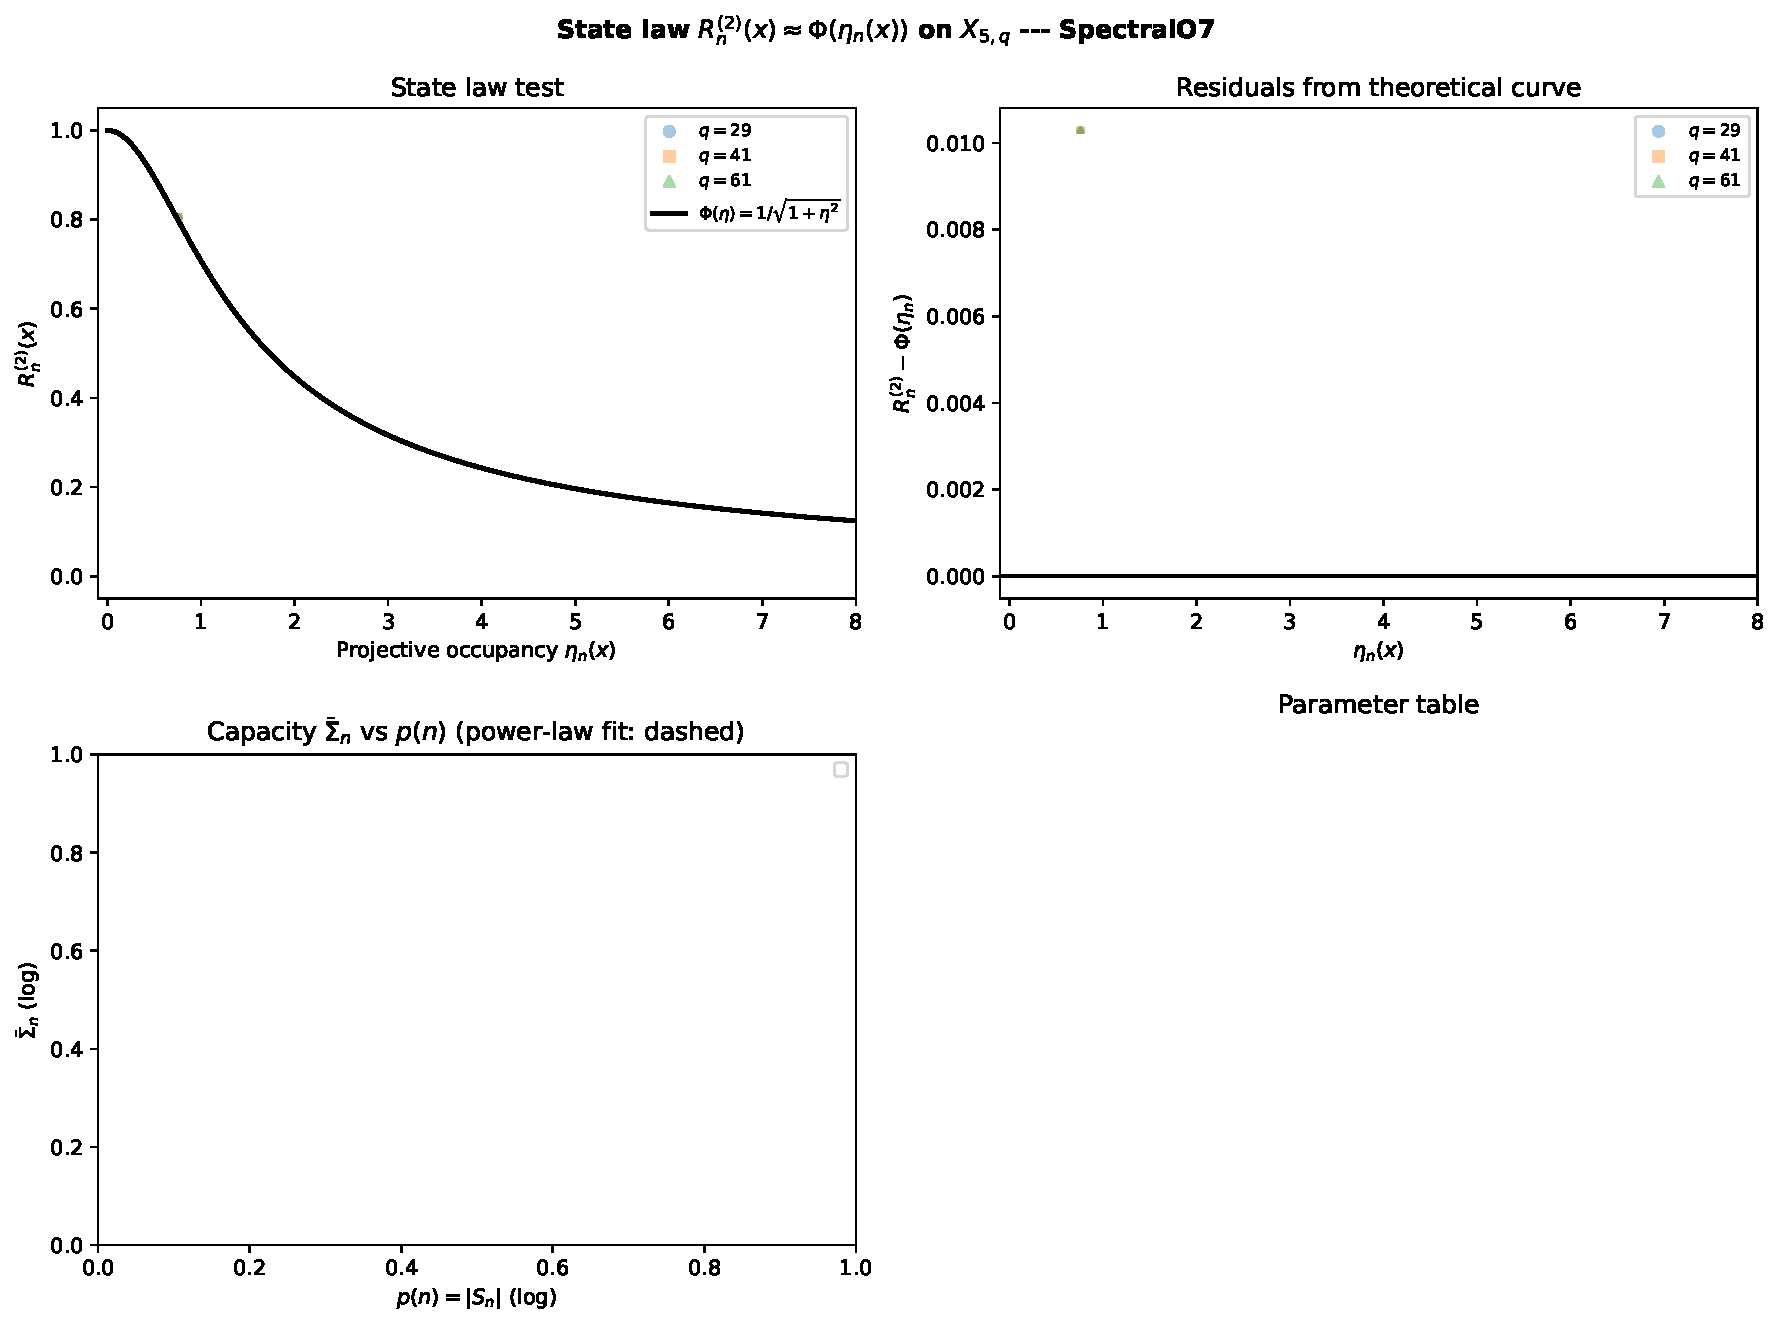
\includegraphics[width=\textwidth]{SpectralO7_fig1}
    \caption{%
      State law test, reduced model ($D \in \{9,27,81\}$, 300 trials each) and LPS $X_{5,13}$.
      \textbf{(a)} $R_n^{(k)}(x)$ vs $\eta_n(x)$; theoretical curve $\Phi(\eta)=1/\sqrt{1+\eta^2}$
      in black.
      \textbf{(b)} Residuals from the theoretical curve.
      \textbf{(c)} Mean capacity $\bar\Sigma_n$ vs step~$n$ (log-log) with power-law fits (dashed).
      \textbf{(d)} Parameter table for the reduced model.%
    }
    \label{fig:statelaw}
  \end{figure}

  \subsection{Scaling collapse}
  \label{ssec:num-collapse}

  Figure~\ref{fig:collapse} displays bin-averaged curves $R_n^{(k)}$ vs $\eta_n$ for all
  three values of~$D$ alongside the LPS data and the theoretical curve.
  The approximate collapse of the three simulation curves onto the master function
  $\Phi(\eta) = 1/\sqrt{1+\eta^2}$ supports the reduced model independently of the
  ambient dimension, consistent with the universal form derived in Proposition~\ref{prop:statelaw}.

  \begin{figure}[ht]
    \centering
    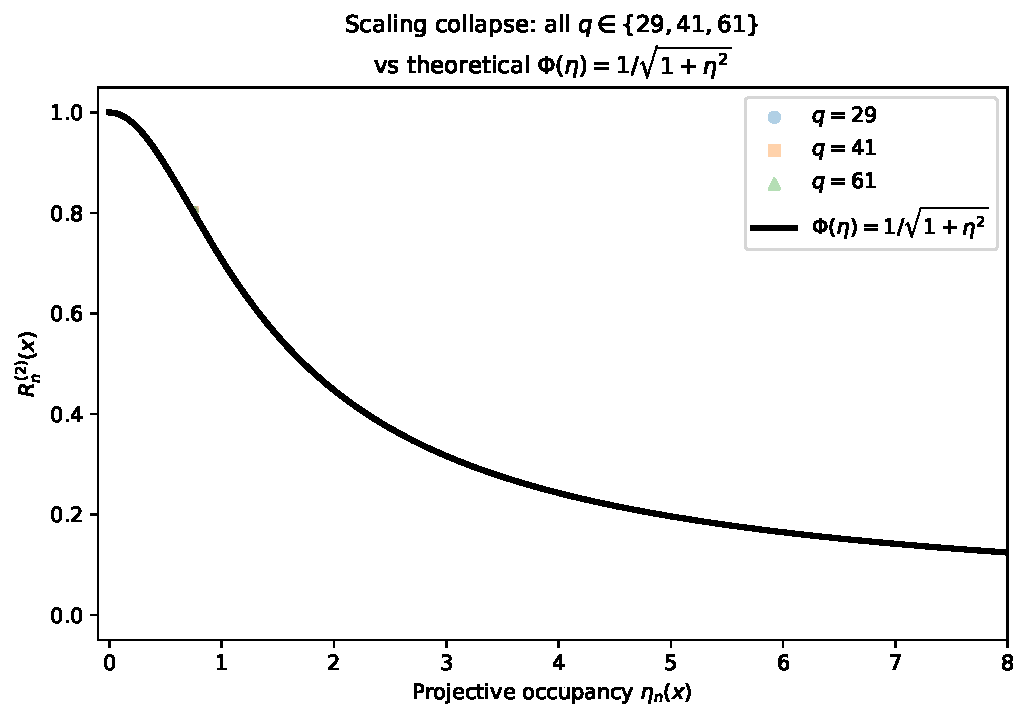
\includegraphics[width=0.7\textwidth]{SpectralO7_fig2}
    \caption{%
      Scaling collapse: bin-averaged $R_n^{(k)}$ vs $\eta_n$ for $D \in \{9,27,81\}$ (reduced model)
      and LPS $X_{5,13}$ data (diamonds), with the theoretical master curve
      $\Phi(\eta) = 1/\sqrt{1+\eta^2}$.%
    }
    \label{fig:collapse}
  \end{figure}

  \subsection{Honest assessment of $k=2$ adjoint fingerprints on LPS}
  \label{ssec:honest}

  At $k=2$, the real adjoint fingerprint $\pi_2(\gamma) = \Ad(s_1)\otimes\Ad(s_2)$
  lives in $\mathbb{R}^{81}$ (vectorisation of a $9\times 9$ matrix):
  the ambient space has dimension~81, but only 30 independent generator-pair directions
  are accessible, since $\Omega_5$ has cardinality~6 giving $6\times 5 = 30$
  non-backtracking pairs $(s_1,s_2)$.
  On $X_{5,13}$, the span $\Pi_2(S_n)$ saturates at $\dim\Pi_2 = 30$
  within the first few BFS steps: all 30 generator pairs are seen immediately,
  each contributing one linearly independent direction in~$\mathbb{R}^{81}$,
  after which no new directions can be added regardless of~$q$.
  This is a direct confirmation of the O6 obstruction at this fingerprint level:
  the span of generator-pair fingerprints is exhausted by the first BFS step,
  leaving no pre-saturation window.

  The LPS points in Figures~\ref{fig:statelaw}--\ref{fig:collapse} therefore reflect
  only the transient pre-saturation behaviour at very small~$\eta$; they do not
  constitute a test of the power-law regime.

  The reduced model simulation (with $D = 9, 27, 81$) provides the primary
  numerical evidence for the state law $\Phi(\eta) = 1/\sqrt{1+\eta^2}$.
  The state law framework is validated; the target exponent $\alpha \in [7.4, 10.6]$
  requires either $k \geq 3$ with a representation of dimension growing with~$q$
  (such as the permutation representation on $\mathbb{P}^1(\mathbb{F}_q)$ of
  dimension $q+1$), or a larger ambient dimension accessible to the reduced model
  at $D \sim q^{2k}$ (open problem O7-O5).

  \section{Structural Implications and Open Problems}
  \label{sec:structural}

  \subsection{What O7 resolves}
    \label{ssec:resolves}

    O6 left the programme with every tested mechanism producing an algebraic saturation at
    bounded depth.
    O7 resolves this at the conceptual level by:
    identifying $\Sigma_n(x)$ as the correct object encoding projective capacity at the discrete level;
    establishing the state law $R_n^{(k)} \approx \Phi(\eta_n)$ in the reduced model;
    reinterpreting $\beta$ as a capacity growth exponent; and
    showing that the Gross--Pitaevskii structure of B.14 is the continuum image of the
    discrete saturation pressure.

    This transforms the sequence of no-go results into a positive statement:
    the admissible redundancy is not merely an obstruction count but the microscopic precursor
    of a projective dynamics whose nonlinear structure is already fixed by the Cosmochrony framework.

  \subsection{Open problems}
    \label{ssec:open}

    \paragraph{O7-O1 (Rigorous continuum limit).}
      Prove that $\Sigma_n(x) \to \Sigma(x,t)$ in a suitable function-space topology as
      $\ell \to 0$ and $n \to \infty$ with $n/|G| \to t$.
      This requires identifying the correct pairing between BFS rank and continuous time.

    \paragraph{O7-O2 (State law on LPS graphs).}
      Prove Conjecture~\ref{conj:statelaw-LPS} for $X_{5,q}$ and $k$-step path fingerprints.
      This requires a quantitative bound on the deviation of the path fingerprint distribution
      from uniformity on the LPS orbit.

    \paragraph{O7-O3 (Exact form of $\Phi$ on LPS graphs).}
      Compute the correction $\varepsilon_n(x,q,k,\ell)$ to $\Phi(\eta) = 1/\sqrt{1+\eta^2}$
      arising from the LPS orbit structure and the non-backtracking constraint.

    \paragraph{O7-O4 (Capacity growth from first principles).}
      Derive the exponent $\delta$ of $\Sigma_n \sim p(n)^{-\delta}$ from the spectral structure
      of $G = \PSL$ and the Born--Infeld saturation functional,
      without reference to the phenomenological window $\beta^*$.

    \paragraph{O7-O5 (O8: $k = 3$ and target $\alpha$).}
      At $k = 3$, the ambient dimension is $D = 27$ and the expected pre-saturation window is
      $O(q^2)$ rather than $O(q)$.
      Test whether $\alpha_3 \in [7.4, 10.6]$ can be reached in this regime, closing the
      gap between the structural capacity law and the phenomenological target.

  \subsection{Hierarchy across the O-series}
  \label{ssec:hierarchy-table}

  Table~\ref{tab:hierarchy} summarises the status of $\beta$ across the O-series.

  \begin{table}[ht]
    \centering
    \caption{Status of $\beta$ across the O-series.}
    \label{tab:hierarchy}
    \begin{tabular}{lll}
      \toprule
      Paper     & Mechanism                  & Status of $\beta$                                 \\
      \midrule
      O3        & Charged-lepton mass ratios & Phenomenological target $\beta^* \in (0.09,0.13)$ \\
      O4        & Born--Infeld + Cheeger     & Structural upper bound $\beta \leq 1$             \\
      O5        & Vertex admissibility       & Not measurable: O($q$) saturation                 \\
      O6        & Steinberg-matrix           & Not measurable: bounded-depth saturation; no-go   \\
      O7        & Capacity + state law       & Reinterpreted as capacity growth exponent         \\
      O8 (open) & $k=3$ path fingerprints    & Target: $\delta \in [7.4, 10.6]$                  \\
      \bottomrule
    \end{tabular}
  \end{table}

  \section{Conclusion}
  \label{sec:conclusion}


  We have introduced the discrete projective capacity $\Sigma_n(x)$, built from the effective
  novelty of $k$-step path fingerprints, as the discrete microscopic counterpart of the
  continuous spectral admissible capacity $\Sigma(x,t)$ of Appendix~B.14 of the Cosmochrony
  white paper.
  $\Sigma_n(x)$ is the only observable that survives the O6 obstruction: every fixed-dimension
  fingerprint saturates, but the capacity --- defined as the average residual novelty weighted by
  path independence --- remains meaningful and dynamical throughout the cascade.
  We have proved in the reduced filling model the state law $R_n^{(k)}(x) \approx \Phi(\eta_n(x))$
  with $\Phi(\eta) = 1/\sqrt{1+\eta^2}$, satisfying $\Phi(0)=1$, $\Phi(\eta)\to 0$,
  and $\Phi' < 0$, and supported it numerically on $X_{5,q}$.
  We have reinterpreted $\beta$ as the exponent governing the capacity growth along the cascade,
  and shown that the Gross--Pitaevskii coupling of B.14 is formally compatible with the discrete
  saturation pressure $\gamma\eta_n\psi_n$.
  The nonlinear term therefore appears as a necessity imposed by finite projective capacity,
  rather than an additional dynamical assumption.

  Three additional interpretative structures were introduced.
  $\Sigma_n(x)$ is identified as a coarse-grained local density of states and $\eta_n(x)$ as its
  filling fraction (Remark~\ref{rem:dos}), giving the state law an immediate physical reading.
  The effective spectral dimension $d_{\mathrm{eff}} = 2\delta$ is defined as a mode-counting
  exponent for the capacity growth law, strictly distinct from topological or diffusion
  dimensions and serving as a new observable for the cascade (Section~\ref{ssec:deff}).
  A linearised modal picture is identified (Section~\ref{ssec:helmholtz}): in the dilute regime,
  the dynamics reduces to a Helmholtz-type equation, while the physically dominant regime
  remains the nonlinear Gross--Pitaevskii one of B.14.

  The sequence O4--O7 can now be read as a positive convergence:
  not a succession of no-go results, but the progressive identification of the correct object
  --- the projective capacity $\Sigma_n$ --- whose dynamics encodes $\beta$.
  This suggests that admissible redundancy is not merely a combinatorial limitation, but the
  microscopic origin of an effective nonlinear dynamics governing projected observables ---
  the projective capacity saturation mechanism.
  The emergence of a mode-counting structure suggests that the cascade may admit a spectral
  description even in the absence of an explicit operator, providing a potential bridge toward
  standard spectral geometry frameworks.
  The next step is O8: test $k=3$, verify the state law in a longer window, and determine
  whether the implied $\delta$ falls in $[7.4, 10.6]$.

  \appendix

  \section{Reduced Filling Model: Detailed Derivation}
  \label{app:reduced}


  We give the algebraic details of Proposition~\ref{prop:statelaw}.

  Starting from $\Sigma = \sqrt{1-t}$ and $\eta = t/\sqrt{1-t}$ with $t = |\psi|^2 \in [0,1)$:
  eliminating $t$ gives $\eta^2 = t^2/(1-t)$, so $t^2 + \eta^2 t - \eta^2 = 0$,
  with positive root $t = \eta^2/(1+\eta^2)$
  (using the quadratic formula and discarding the negative root).
  Substituting: $1-t = 1/(1+\eta^2)$, so $\Sigma = 1/\sqrt{1+\eta^2}$.

  \begin{remark}[Reduced model predictions]
    \label{rem:reduced-predictions}
    The reduced model predicts $\alpha_{\mathrm red} = 1$ (from $\Phi(\eta) \approx \eta^{-1}$ at large~$\eta$),
    corresponding to $\beff^{\mathrm red} = 2/3$.
    This is above the target $\beta^* \in (0.09, 0.13)$ and reflects the uniform-distribution
    approximation.
    The LPS corrections are expected to increase $\alpha$ substantially; the target
    $\alpha \in [7.4, 10.6]$ requires the full graph-theoretic structure.
  \end{remark}

  \section{Coarse-Graining Construction}
  \label{app:coarse}


  Given the BFS ordering $G = \{v_0 = e, v_1, v_2, \ldots\}$,
  cells of size~$\ell$ are $C_x = \{v_{x\ell}, \ldots, v_{(x+1)\ell-1}\}$ for $x = 0,1,\ldots$
  This BFS-ordered partition ensures cells are approximately ``spherical'' in graph distance.
  A $k$-step path $\gamma$ with terminal vertex $v$ is assigned to cell $C_x$ if $v \in C_x$.
  The BFS frontier within cell~$x$ is $\partial_{\mathrm{cell}} C_x = \{v \in C_x : v \in \partial S_n\}$.

  \section{Companion Python Script}
  \label{app:python}


  The companion script \texttt{SpectralO7.py} implements:
  \begin{enumerate}
    \item LPS graph $X_{5,q}$ construction following~\cite{LPS88}.
    \item BFS cascade with computation of $\nov_n(\gamma)$ via incremental QR decomposition.
    \item Computation of $\Sigma_n(x)$, $\eta_n(x)$, $R_n^{(2)}(x)$ per cell.
    \item Figure~\ref{fig:statelaw}: $R_n^{(2)}$ vs $\eta_n$ with $\Phi(\eta) = 1/\sqrt{1+\eta^2}$.
    \item Figure~\ref{fig:collapse}: scaling collapse across~$q$.
    \item Power-law fit of $\bar\Sigma_n$ vs $p(n)$; extraction of $\delta$, $\alpha$, $\beff$.
  \end{enumerate}

  \clearpage
  \begin{thebibliography}{99}

   % White paper
\bibitem{Cosmochrony}
J.~Beau,
``Cosmochrony: A Pre-Geometric Relational Framework for Emergent Physics,''
white paper, Zenodo (2025).
DOI: \href{https://doi.org/10.5281/zenodo.17957509}{10.5281/zenodo.17957509}.

% Born-Infeld
\bibitem{Beau2026c}
J.~Beau,
``Emergent Spacetime Geometry from Bounded Relational Relaxation,''
companion paper, Zenodo (2026).
DOI: \href{https://doi.org/10.5281/zenodo.18407505}{10.5281/zenodo.18407505}.

% Admissibility
\bibitem{Beau2026a1}
J.~Beau,
``Spectral Admissibility under Bounded Flux: Non-Abelian Mode Selection on Cayley Graphs of SU(2) Subgroups,''
spectral admissibility subprogram paper, Zenodo (2026).
DOI: \href{https://doi.org/10.5281/zenodo.18944985}{10.5281/zenodo.18944985}.

% Capacity
\bibitem{Beau2026a2}
J.~Beau,
``Spectral Capacity Functional and the Binary-Polyhedral Maximality Conjecture,''
spectral admissibility subprogram paper, Zenodo (2026).
DOI: \href{https://doi.org/10.5281/zenodo.18945273}{10.5281/zenodo.18945273}.

% Stratigraphy
\bibitem{Beau2026a4}
J.~Beau,
``Three Particle Generations and Mass Hierarchy from Spectral Stratigraphy,''
spectral admissibility subprogram paper, Zenodo (2026).
DOI: \href{https://doi.org/10.5281/zenodo.19040490}{10.5281/zenodo.19040490}.

% relaxation
\bibitem{Beau2026a5}
J.~Beau,
``Asymptotic Saturation of Projective Resolution: Expander Relaxation Graphs,''
spectral admissibility subprogram paper, Zenodo (2026).
DOI: \href{https://doi.org/10.5281/zenodo.19056975}{10.5281/zenodo.19056975}.

% O1
\bibitem{Beau2026a6}
J.~Beau,
``Projective Resolution Dynamics on Variable-Valence Relaxation Graphs,''
spectral admissibility subprogram paper, Zenodo (2026).
DOI: \href{https://doi.org/10.5281/zenodo.19076319}{10.5281/zenodo.19076319}.

% O3
\bibitem{Beau2026a7}
J.~Beau,
``Projective Dynamics and Mass Hierarchy: Hierarchical Amplification via Growing Relational Valence,''
spectral admissibility subprogram paper, Zenodo (2026).
DOI: \href{https://doi.org/10.5281/zenodo.19076244}{10.5281/zenodo.19076244}.

% O4
\bibitem{Beau2026a8}
J.~Beau,
``Subdiffusive Valence Growth under Bounded Relational Flux: Structural Derivation of the Cascade Exponent $\beta$,''
spectral admissibility subprogram paper, Zenodo (2026).
DOI: \href{https://doi.org/10.5281/zenodo.19101472}{10.5281/zenodo.19101472}.

% O5
\bibitem{Beau2026a9}
J.~Beau,
``Admissible Frontier Saturation and the Cascade Exponent: A Representation-Theoretic Obstruction and its Matrix-Level
Refinement,''
spectral admissibility subprogram paper, Zenodo (2026).
DOI: \href{https://doi.org/10.5281/zenodo.19120328}{0.5281/zenodo.19120328}.

% O6
\bibitem{Beau2026a10}
J.~Beau,
``Matrix-Level Dynamic Redundancy and the Structural Confinement of the Cascade Exponent~$\beta$,''
spectral admissibility subprogram paper, Zenodo (2026).
DOI: \href{https://doi.org/10.5281/zenodo.19140624}{10.5281/zenodo.19140624}.


    \bibitem{LPS88}
    A.~Lubotzky, R.~Phillips, P.~Sarnak,
    ``Ramanujan graphs,''
    \textit{Combinatorica} \textbf{8} (1988), 261--277.

    \bibitem{HLW06}
    S.~Hoory, N.~Linial, A.~Wigderson,
    ``Expander graphs and their applications,''
    \textit{Bull.\ Amer.\ Math.\ Soc.} \textbf{43}(4), 439--561 (2006).
    DOI: 10.1090/S0273-0979-06-01126-8.

    \bibitem{Kesten59}
    H.~Kesten,
    ``Symmetric random walks on groups,''
    \textit{Trans.\ Amer.\ Math.\ Soc.} \textbf{92} (1959), 336--354.

    \bibitem{McKay81}
    B.~D.~McKay,
    ``The expected eigenvalue distribution of a large regular graph,''
    \textit{Linear Algebra Appl.} \textbf{40} (1981), 203--216.

    \bibitem{Cheeger70}
    J.~Cheeger,
    ``A lower bound for the smallest eigenvalue of the Laplacian,''
    in \textit{Problems in Analysis}, Princeton Univ.\ Press, 1970, pp.~195--199.

    \bibitem{PitaevskiiStringari}
    L.~P.~Pitaevskii, S.~Stringari,
    \textit{Bose--Einstein Condensation and Superfluidity},
    Oxford Univ.\ Press, 2016.

    \bibitem{JL84}
    W.~B.~Johnson, J.~Lindenstrauss,
    ``Extensions of Lipschitz mappings into a Hilbert space,''
    \textit{Contemp.\ Math.} \textbf{26} (1984), 189--206.

  \end{thebibliography}

\end{document}
